\documentclass[border=10pt]{standalone}
\usepackage[svgnames]{xcolor}
\usepackage{amsmath}
\usepackage{pgfplots}
\pgfplotsset{compat=newest}
\usepackage[sfdefault]{FiraSans}
\usepackage{FiraMono}
\renewcommand*\familydefault{\sfdefault}
\begin{document}
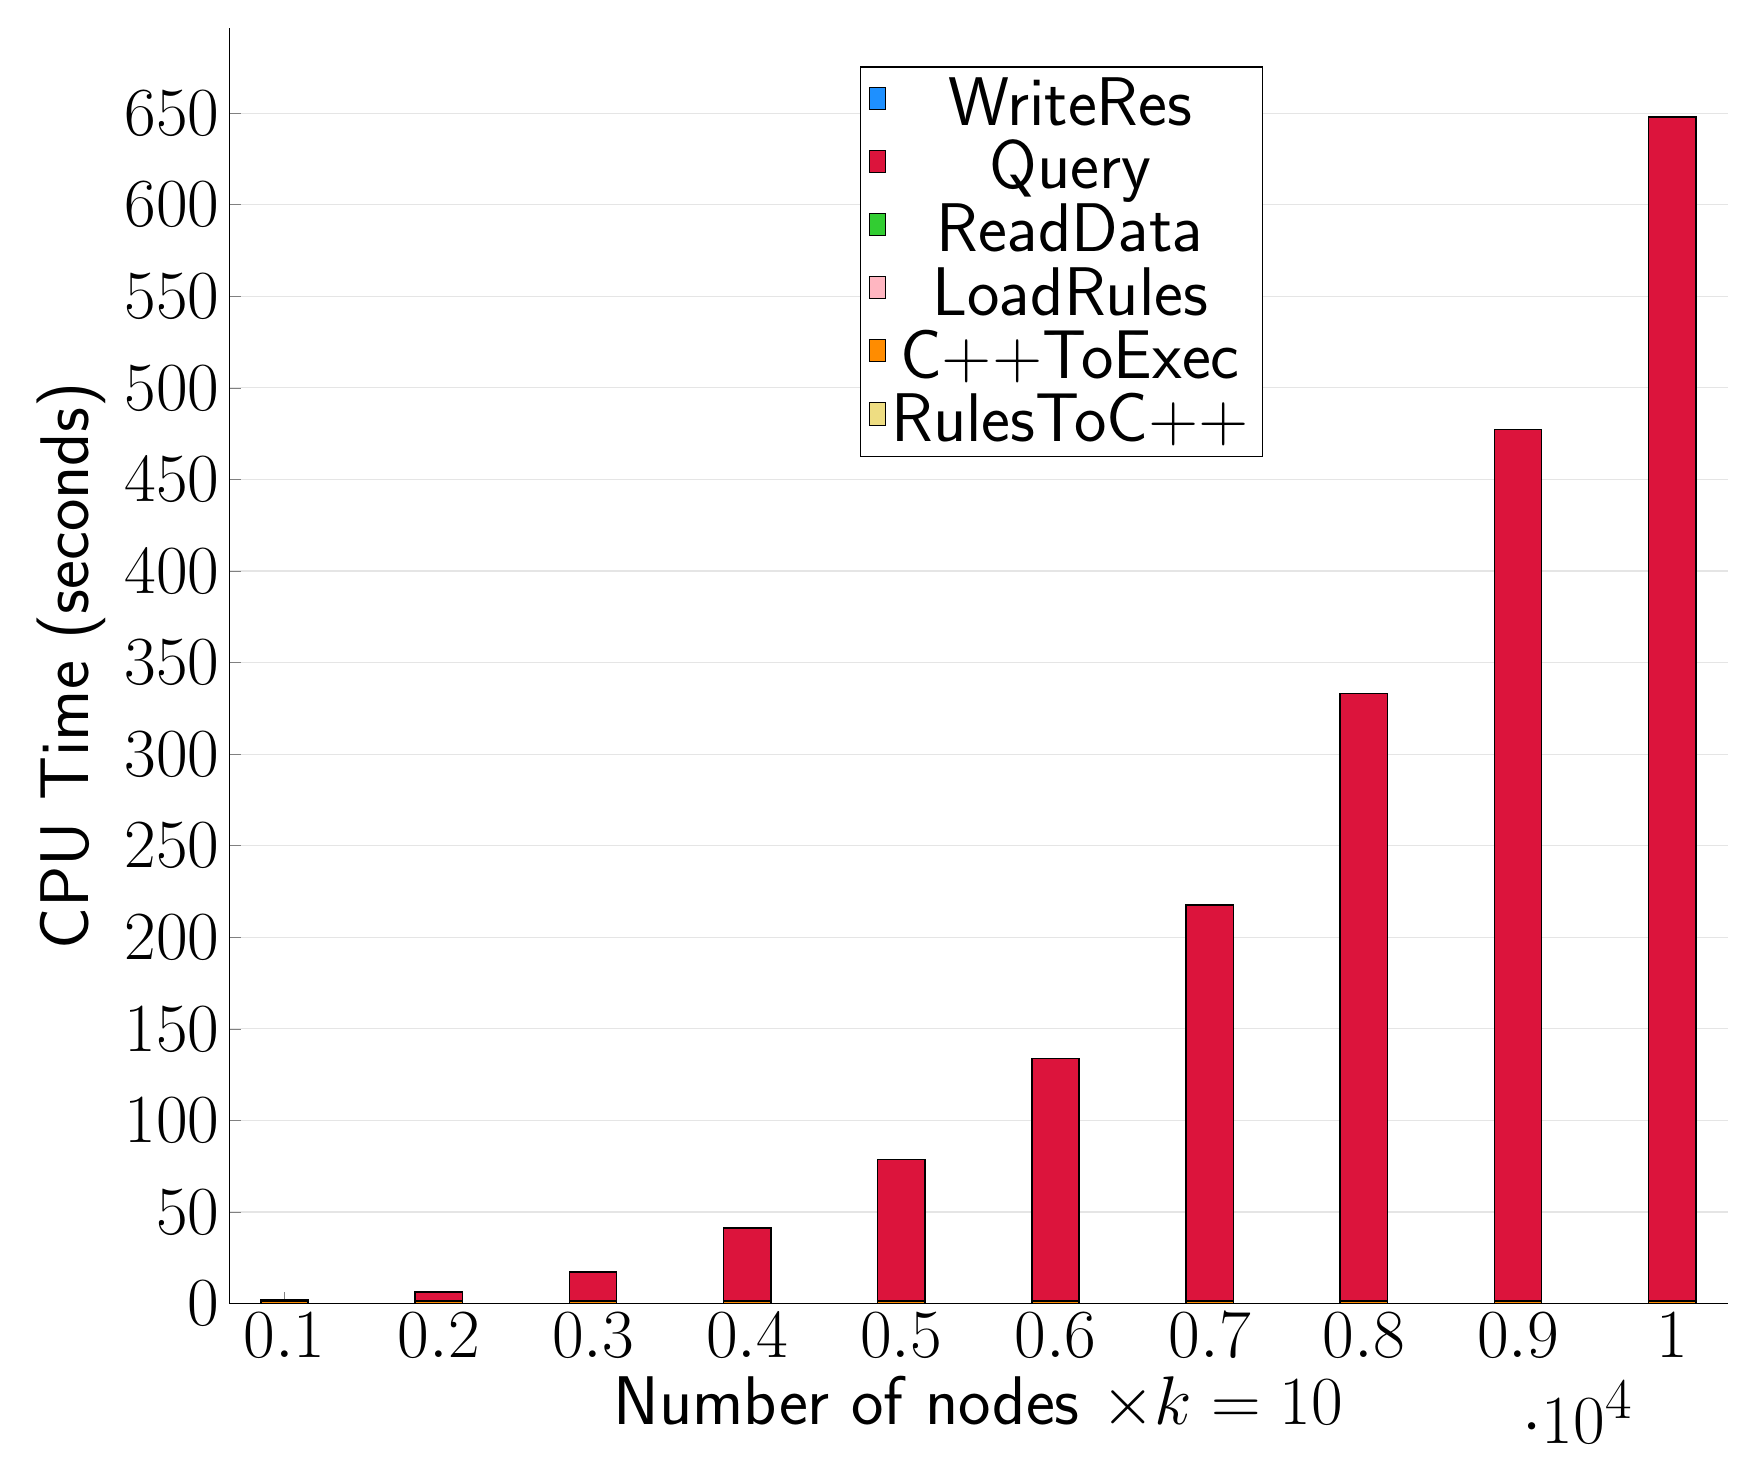
\begin{tikzpicture}
\begin{axis}[
   ybar stacked,
   width=1.7\textwidth,
   bar width=0.6cm,
   ymajorgrids, tick align=inside,
   major grid style={draw=gray!20},
   xtick=data,
   ymin=0, ymax=696.3414,
   axis x line*=bottom,
   axis y line*=left,
   enlarge x limits=0.04,
   legend style={
       at={(0.69, 0.97)},
       anchor=north east,
       legend columns=1,
       font=\Huge,
   },
   ylabel={CPU Time (seconds)},
   xlabel={Number of nodes $\times k=10$},
   label style={font=\Huge},
   tick label style={font=\Huge},
]
\addlegendimage{fill=DodgerBlue, draw=black, line width=0.2pt}
\addlegendentry{WriteRes}
\addlegendimage{fill=Crimson, draw=black, line width=0.2pt}
\addlegendentry{Query}
\addlegendimage{fill=LimeGreen, draw=black, line width=0.2pt}
\addlegendentry{ReadData}
\addlegendimage{fill=LightPink, draw=black, line width=0.2pt}
\addlegendentry{LoadRules}
\addlegendimage{fill=DarkOrange, draw=black, line width=0.2pt}
\addlegendentry{C++ToExec}
\addlegendimage{fill=LightGoldenrod, draw=black, line width=0.2pt}
\addlegendentry{RulesToC++}
\addplot +[fill=LightGoldenrod, draw=black, line width=0.55pt] coordinates {
(1000, 0.008000000000000002)
(2000, 0.010000000000000002)
(3000, 0.010000000000000002)
(4000, 0.006000000000000001)
(5000, 0.004000000000000001)
(6000, 0.0020000000000000005)
(7000, 0.0020000000000000005)
(8000, 0.0)
(9000, 0.0020000000000000005)
(10000, 0.004000000000000001)
};
\addplot +[fill=DarkOrange, draw=black, line width=0.55pt] coordinates {
(1000, 1.53)
(2000, 1.5299999999999998)
(3000, 1.528)
(4000, 1.528)
(5000, 1.534)
(6000, 1.53)
(7000, 1.536)
(8000, 1.532)
(9000, 1.534)
(10000, 1.56)
};
\addplot +[fill=LightPink, draw=black, line width=0.55pt] coordinates {
(1000, 0.0001584)
(2000, 0.0001582)
(3000, 0.0001562)
(4000, 0.0001382)
(5000, 0.00016199999999999998)
(6000, 0.00016959999999999998)
(7000, 0.00018879999999999998)
(8000, 0.00017260000000000002)
(9000, 0.00017479999999999997)
(10000, 0.000188)
};
\addplot +[fill=LimeGreen, draw=black, line width=0.55pt] coordinates {
(1000, 0.0036542)
(2000, 0.006639600000000001)
(3000, 0.0088608)
(4000, 0.0117924)
(5000, 0.0150004)
(6000, 0.0172298)
(7000, 0.0203124)
(8000, 0.020707200000000002)
(9000, 0.022619400000000005)
(10000, 0.026368400000000004)
};
\addplot +[fill=Crimson, draw=black, line width=0.55pt] coordinates {
(1000, 0.6166638000000001)
(2000, 4.815466)
(3000, 15.850519999999998)
(4000, 39.750659999999996)
(5000, 77.11266)
(6000, 132.3686)
(7000, 216.15840000000003)
(8000, 331.65520000000004)
(9000, 475.62119999999993)
(10000, 646.3414)
};
\addplot +[fill=DodgerBlue, draw=black, line width=0.55pt] coordinates {
(1000, 0.000332)
(2000, 0.0004094)
(3000, 0.0003776)
(4000, 0.0003926)
(5000, 0.0004546)
(6000, 0.00042839999999999995)
(7000, 0.00046899999999999996)
(8000, 0.00047279999999999995)
(9000, 0.0005234)
(10000, 0.0005536)
};
\end{axis}
\end{tikzpicture}

\end{document}
